\chapter{Bosonization of Bosons}
Bosonization is a non-perturbative technique belonging to the family of quantum field theory techniques. It is a valuable tool for studying strongly correlated many-body systems. The process of
bosonization entails identifying an effective bosonic system model that is analogous to the original system model within a specified energy interval. \\ \\

\newpage
In this chapter the bosonization technique is reviewed. The technique allows us not only to represent fermionics fields but also bosonics ones as shown in this chapter . This chapter attempts to be self-contained, introduces the derivation of the bosonic identity and a brief application with reticular spinless bosons helping us to paave the path for the next step which is the Bose-Hubbard model for  spin-1 particles.



\textcolor{UVred}{Hola profe, con qué puedo alimentar este pequeño preámbulo del capítulo. Se me ocurre abordar un poco más en los resultados que se obtienen al aplicar la técnica al sistema de bosones retículares pero no sé que tan apropiado sea o abordar más en el modelo de Bose-Hubbard}\\ \\




\section{Heuristic Bosonization}
Nuestro objetivo es describir el proceso de bosonización de un sistema de particulas unidimensionales fuertemente correlacionadas. Para eso, el primer paso que se debe realizar es tener familiaridad con el sistema que tenemos, consideremos un sistema de bosones unidimensionales sin espin libres que se encuentren libres y que su relación de dispersión es cosenoidal y dada por la siguiente ecuación:
\begin{equation} \label{2_H_free_bosons}
    \hat{H} = -2t\cos{\left(\frac{2\pi}{L} k\right)} \hat{b}^{\dagger}_{k}\hat{b}^{}_{k},
\end{equation}
al graficar esta relación de dispersión en el espacio de momento se obtiene la figura\ref{2_fig_bosonic_chirial}.

\begin{figure}[h!]
    \centering
    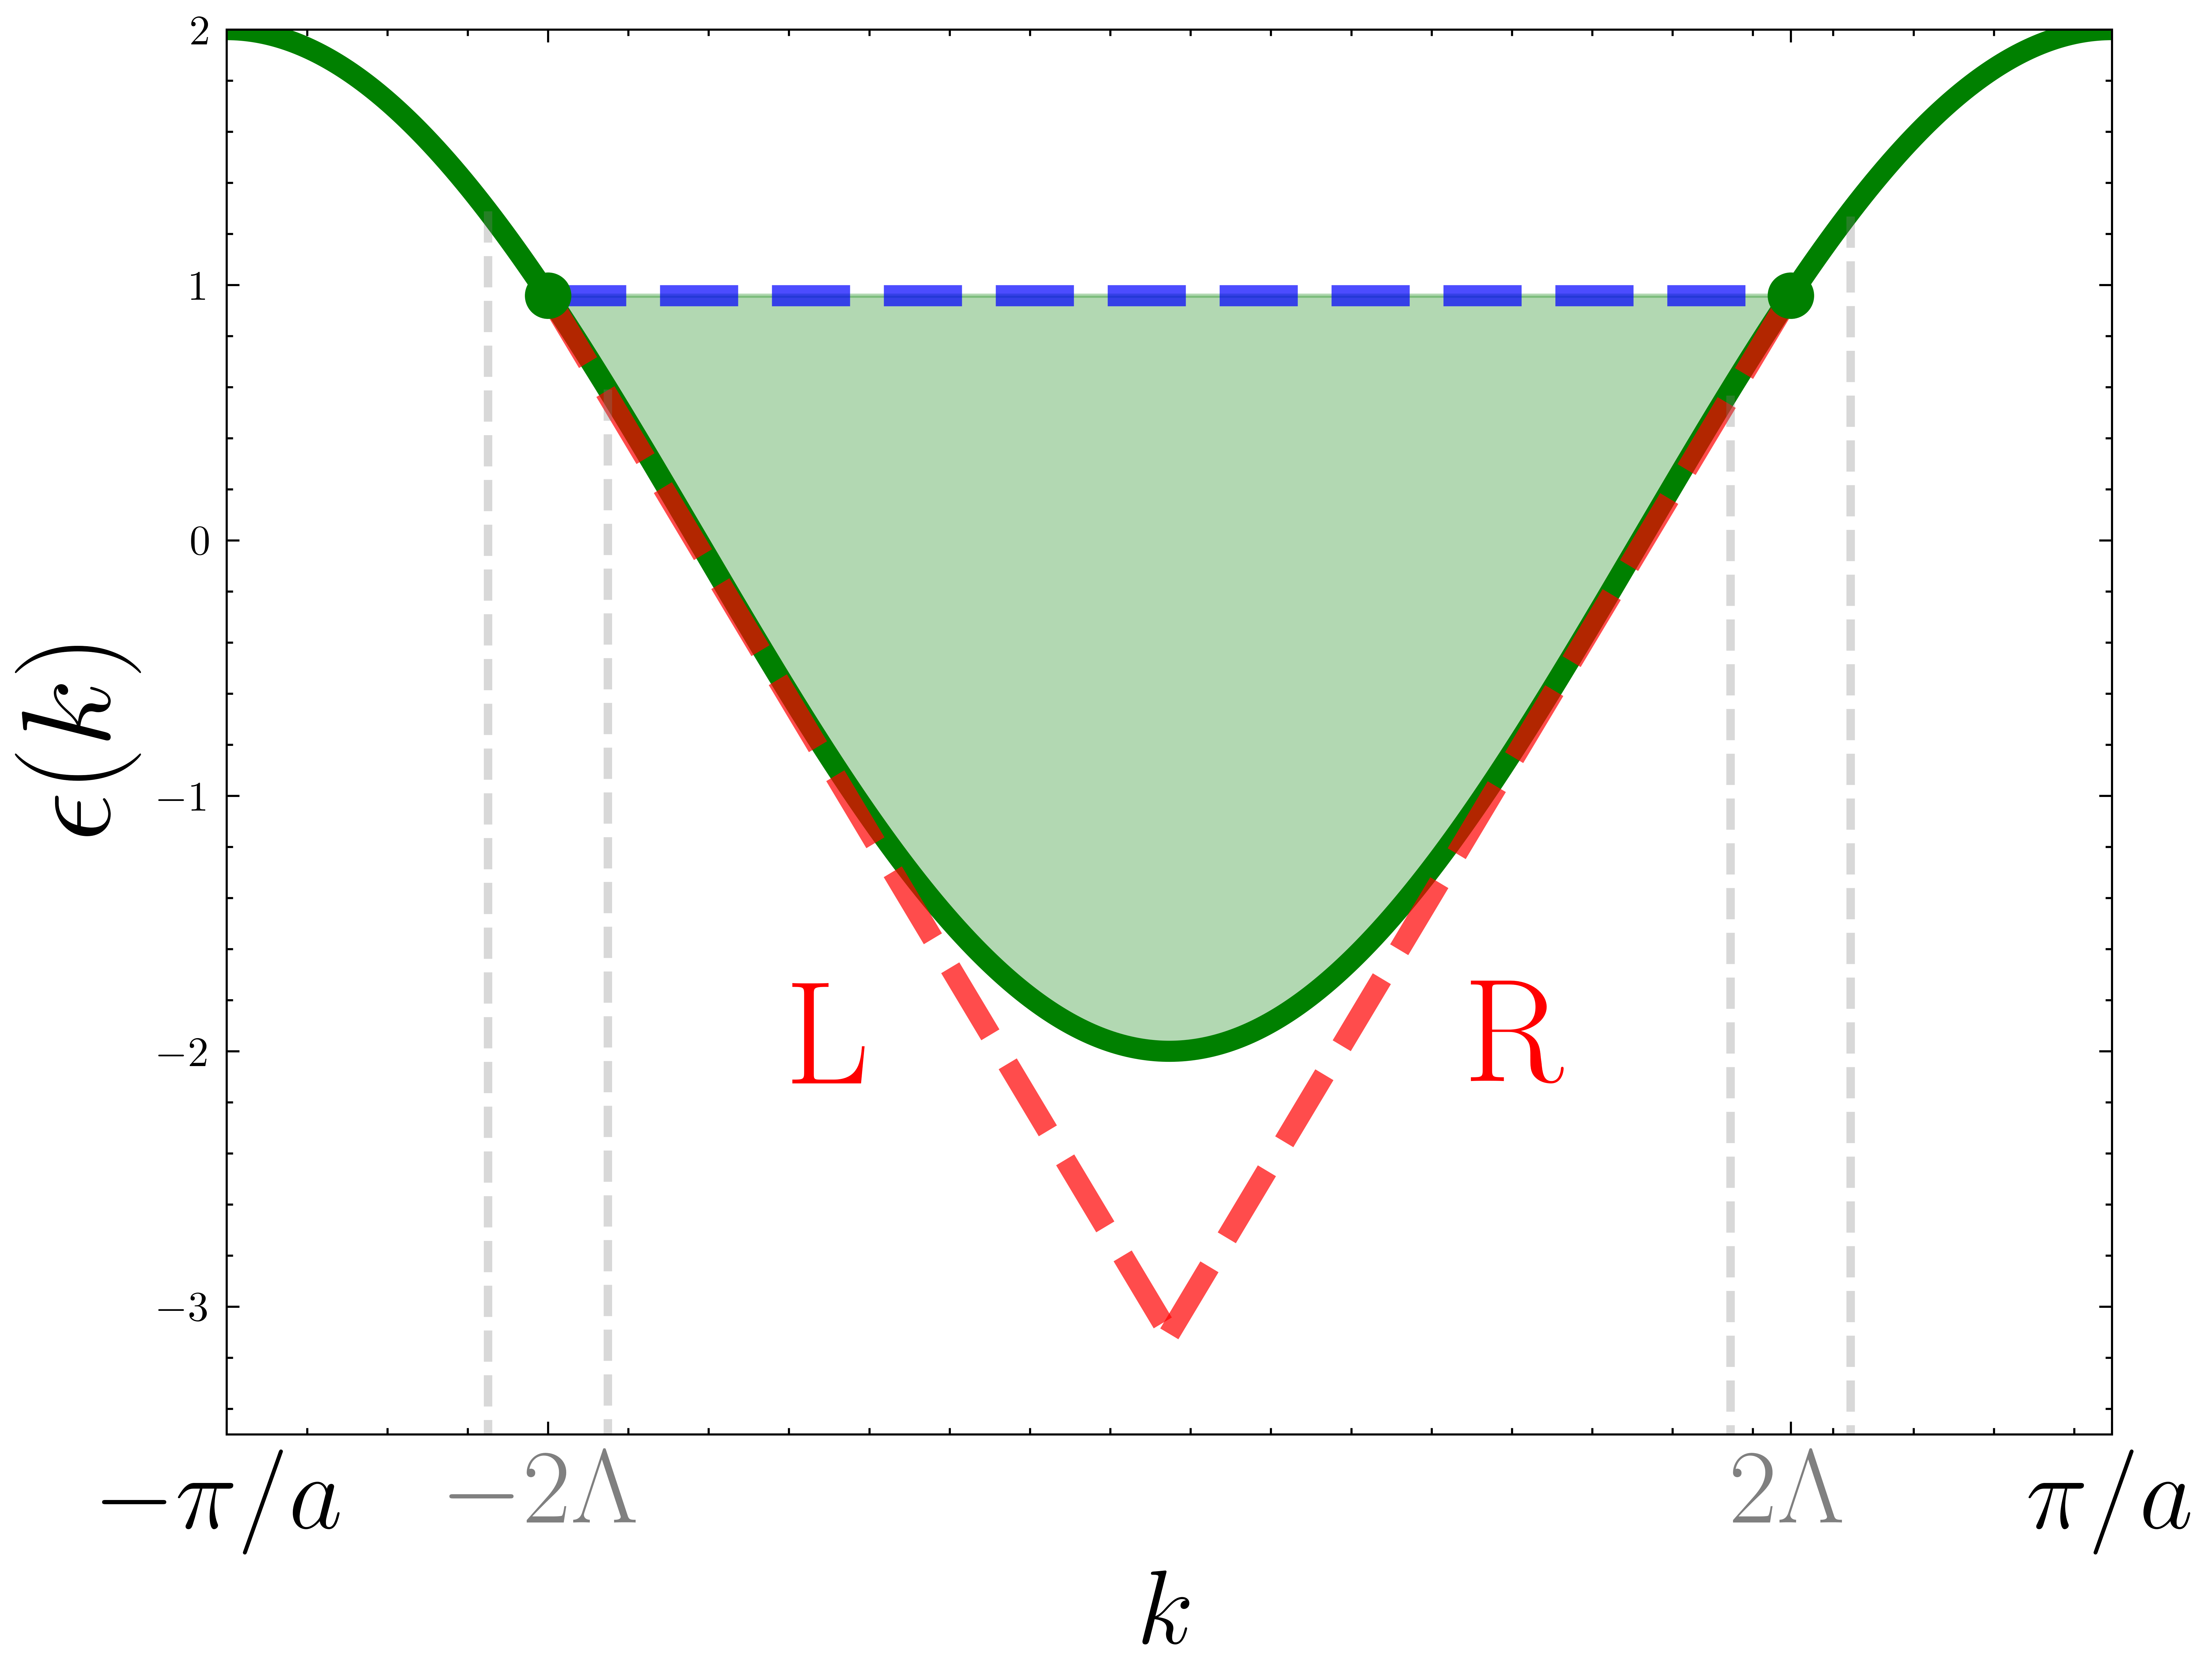
\includegraphics[scale=0.5]{Figures/Chapter 2/Grafica_Bosonization_Relation.png}
    \caption{Relacion de dispersión de un hamiltoniano de bosones libres.}
    \label{2_fig_bosonic_chirial}
\end{figure}
Es claro, que en la figura (\ref{2_fig_bosonic_chirial}) se ha pintado dos lineas que coinciden exactamente con el valor de la relación de dispersión para cuando observamos el sistema dentro de un intervalo $\Gamma$ especifico. Estas dos lineas nos permiten aproximar de manera exacta el sistema real descrito por el (\ref{2_H_free_bosons}) a un \textit{sistema efectivo} compuesto por dos sistemas lineales, que si bien no nos permiten describir el sistema real para todos los valores de momento, es exacto cuando nos encontramos dentro del intervalo mencionado. Esto indica que los operadores de destrucción y creación que diagonalizaban la relación de dispersión de la ecuación (\ref{2_H_free_bosons}) 
\begin{equation} \label{eq_a_momentum_operator}
\begin{aligned}
     \hat{b}(k)=\theta(k) \hat{\varphi}_{R}(k)+\theta(-k) \hat{\varphi}_{L}(k) \\
     \hat{b}^{\dagger}(k)=\theta(k) \hat{\varphi^{\dagger}}_{R}(k)+\theta(-k) \hat{\varphi^{\dagger}}_{L}(k)     
\end{aligned}   
\end{equation}
donde $\theta(k)$ es la función paso y $\hat{\varphi}_{R}(k)$, $\hat{\varphi}_{L}(k)$ son los campos de los operadores quiriales que describen \textit{efectivamente} el sistema. \\ \\
Entender el proceso anterior es esencial, como se puede apreciar en toda la literatura sobre bosonizacion [] siempre se empieza con esta imagen de linealización sobre el espectro de energía. Este es el concepto clave y que puede ser dificil al inicio de digerir.


\subsection{Single branch system.}
Ahora enfoquemonos en una sola rama del sistema que previamente hemos mencionado.


\subsection{Two branch system.}







\newpage
\section{Fields}
As mentioned at the beginning of this chapter, bosonization is a field theory, specifically a quantum field theory. To continue our discussion, it is important to define what we consider a free boson from the point of view of a quantum field theory. In principle, this must be done from a Lagrangian point of view. In the case of a massless bosonic field we have $\hat{\Phi}$:
\begin{equation} \label{2_2_1}
\hat{L_0}=\frac{1}{2} \int \mathrm{~d} x\left[\frac{1}{v}\left(\partial_t \hat{\Phi} (x)\right)^2-v\left(\partial_x  \hat{\Phi} (x)\right)^2\right],
\end{equation}
where $v$ is the Bose particle velocity. The Hamiltonian corresponding to the density would be
\begin{equation} \label{2_2_2}
    \hat{H}_0 = \frac{1}{2} v \big[ \frac{1}{v} (\hat{\Pi})^2
 -v(\partial \phi)^2 \big], 
\end{equation}
with $\hat{\Pi}$ being a conjugate field of $\phi$, the two fields obey the canonical commutation rules:
\begin{equation} \label{2_2_3}
    \big[ \hat{\Phi} (x), \hat{\Pi} (x) \big] = i \delta (x-x^{\prime}).
\end{equation}
The standard expansion for the fields $\hat{\phi}$ and $\hat{\Pi}$ in terms of their modes on an infinite line is given by:   
\begin{equation} \label{2_2_4}
    \hat{\Phi}(x, t)=\sum_{p \neq 0} \sqrt{\frac{1}{2 L|p|}}\left(e^{i\left(p x-|p| v_{E} t\right)} \hat{b}_{p}+\text { h.c. }\right),
\end{equation}
\begin{equation} \label{2_2_5}
   \hat{\Pi}(x, t)=-i \sum_{p \neq 0} \sqrt{\frac{|p|}{2 L}}\left(e^{i\left(p x-|p| v_{E} t\right)} \hat{b}_{p}-\text { h.c. }\right), 
\end{equation}
where $\hat{b}_{p}$ and $\hat{b}^{\dagger}_{p}$ are creation and destruction operators, and must obey the following commutation relation:
\begin{equation} \label{2_2_6}
    [\hat{b}_{p}, \hat{b}^{\dagger}_{p^{\prime}}] = 2\pi \delta (p-p^{\prime}),
\end{equation}
and allows the Hamiltonian to be expressed as follows:
\begin{equation} \label{2_2_7}
    \hat{H} = \int \frac{dk}{2\pi} \omega(k) \hat{b}_{k}^{\dagger} \hat{b}_{k}, 
\end{equation}
where $\omega (k) = v \abs{k}$ The ground (or vacuum) state $\ket{0}$ is destroyed by all operators $\hat{b} (k)$ and has zero energy by convection. It is worth noting and emphasizing that the previous Hamiltonian has a similar form to the one we have been working on from the beginning to visualize our formalism.\\ \\
Similarly, we can express the creation and destruction operators of the normal modes of the system in terms of the bosonic fields we have defined by adding the fields \ref{2_2_4} and \ref{2_2_5} and solving for each one we get:
\begin{equation} \label{2_2_8}
  \hat{b}_{p}  =\frac{-i}{\sqrt{2|p| L}} \int \mathrm{d} x e^{-i p x}\left(\operatorname{sgn}(p) \partial_{x} \hat{\Phi}-\hat{\Pi}\right)  \quad \quad   \hat{b}_{p}^{\dagger}  =\frac{i}{\sqrt{2|p| L}} \int \mathrm{d} x e^{i p x}\left(\operatorname{sgn}(p) \partial_{x} \hat{\Phi}-\hat{\Pi}\right) .
\end{equation}
It is important to define two additional fields, which allow us to work with the dynamics of the system:
\begin{equation} \label{2_2_9}
\hat{\theta}(x, t)=-\sum \frac{\operatorname{sgn}(p)}{\sqrt{2 L|p|}}\left(e^{i\left(p x-v_{E}|p| t\right)} \hat{b}_{p}+\text { h.c. }\right), 
\end{equation}
\begin{equation} \label{2_2_10}
\hat{\phi}_{\alpha}=\sum_{\alpha p>0} \sqrt{\frac{1}{2 L|p|}}\left(e^{i\left(p x-|p| v_{E} t\right)} \hat{b}_{p}+\text { h.c. }\right).
\end{equation}
\textcolor{myred}{Me gustaría añadir aqui unos parrafos hablando de la importancia y la necesidad de estos campos.}
\section{Bosonization Identity}
Now, in order to achieve functionally the bosonization identity with which we will work, we will follow the treatment made in [Ref: Giarmachi], we see that the main objective is to be able to have a bosonization identity that relates the creation and destruction operators of the original system in terms of bosonic fields that allow us to describe the dynamics of the system in a simpler way. To do this, we will change the point of view proposed in the previous sections, we will introduce a small new formalism that maintains the essence of the information, which is that: the current densities of the interactions that arise in the system are of a bosonic character.\\ \\
We can start with a one-dimensional boson (or fermion) system. The density operator for such a system is
\begin{equation} \label{B_I_eq_density}
    \hat{\rho}(x)=\sum_{i} \delta(x-x_{i}),
\end{equation}
where $x_{i}$ is the position of the i-th particle. Suppose that the position $R_{i}^{0}$ is called the "equilibrium position", this position would be the position occupied by the particle if the particles formed a perfect crystalline network, any displacement $u_{i}$ relative to this position is given by:
\begin{equation} \label{2_3_2}
    x_{i}=R_{i}^{0} + u_{i}.
\end{equation}
If we define $\rho_{0}$ as the mean density of the particle system, $d=\rho_{0}^{-1}$ is the distance between the particles. This would allow us to see that the equilibrium position of the i-th particle is:
\begin{equation}\label{2_3_3}
   R_{i}^{0}=di. 
\end{equation}
In order to deal more properly with the equation \eqref{B_I_eq_density}, we introduce the field $\Phi_{l}(x)$ in the same way as Haldane first did [Reference Haldane,1981b]. This field, which is a continuous function in position, takes the value $\hat{\Phi}_{l}(x_{i})=2\pi i$ when the particle is at the i-th position. This allows us to see another way of looking at the number of particles. This is a peculiarity of one-dimensional systems; unlike high-dimensional systems, we can always obtain the number of particles in a unique way, for example, by starting at $x= - \infty$ and contracting from left to right.\\ \\
\textcolor{myred}{Aquí iría otra grafica (2.3) extra que muestre el comportamiento del Campo $\hat{\phi}$ mencionado. } \\ \\
Using the following transformation rule for $\delta$ functions:
\begin{equation} \label{2_3_4}
    \delta(f(x)) = \sum \frac{1}{|f^{\prime}(x_{i})| \delta(x-x_{i})} ,
\end{equation}
we can rewrite the density \eqref{B_I_eq_density} as:
\begin{equation} \label{B_I_eq_rho_2}
    \begin{aligned} 
            \hat{\rho}(x) &=\sum_{i} \delta(x-x_{i}) \\
               &= \sum_{n} | \nabla \hat{ \Phi}_{l}(x)| \delta( \hat{\Phi}_{l}(x)-2\pi n). 
    \end{aligned}
\end{equation}
With the appropriate reference system, as we can see in figure (2.3:To be added), the field $ $ is always a function that increases with x, which allows us to leave aside the absolute value of \eqref{B_I_eq_rho_2}. Using the Posion summation formula, we can rewrite the equation as follows:
\begin{equation} \label{2_3_6}
    \hat{\rho} (x) = \frac{\nabla \hat{\Phi}_{l}(x)}{2\pi} \sum_{p} e^{ip \hat{\Phi}_{x}(x)},
\end{equation}
where $p$ is defined as an integer. It is convenient to define a field $\hat{\Phi}$ relative to the solution of the perfect crystal and introduce it as follows:
\begin{equation} \label{2_3_7}
    \hat{\Phi}_{l}(x) =2\pi \bar{\rho}_{0}x -2 \hat{\Phi}(x). 
\end{equation}
Thus, the density becomes:
\begin{equation} \label{B_I_rho_3}
    \hat{\rho}(x) = \big[\bar{\rho}_{0}-\frac{1}{\pi} \nabla \phi(x
)   \big] \sum_{p} e^{i2p(\pi \bar{\rho}_{0}x - \phi(x
))}.
\end{equation}
Since the density operator commutator commutes at two different locations in the lattice, we see that the fields $\phi_(x)$ commute with themselves. A special case of the equation \eqref{B_I_rho_3} occurs when the density is averaged over a distance large compared to the interparticle distance $d$, all oscillating terms disappear. This occurs when $p=0$, which is the density in this case:
\begin{equation} \label{2_3_8}
    \hat{\rho}(x) = \bar{\rho}_{0}-\frac{1}{\pi} \nabla \phi(x
).   
\end{equation}
This happens in the strongly correlated systems that we study and work on, we see that we can average over a large distance because it is comparable to the distance between particles. This means that these oscillating terms are important and necessary to adequately describe the dynamics of these systems. \\ \\
Following this line of thought we can go deeper by observing the behavior of a bosonic construction operator $\hat{b}^{\dagger}(x)$, we know that these operators can be written as follows:
\begin{equation}\label{B_I_eq_Identity}         
   \hat{b}^{\dagger} (x) = [\hat{\rho}(x)]^{1/2} e ^{-i\hat{\theta} (x)},
\end{equation}
where $\hat{\theta}(x)$ is some operator. It is known that the commutation relation between the creation and destruction operators is of bosonic character, which causes conditions to be imposed within the density operator of the system. As we will see below,
\begin{equation} \label{2_3_9}
    [\hat{b}(x), \hat{b}^{\dagger}(x^{\prime})] = \delta (x-x^{\prime}),
\end{equation}
substituting the information in the equation \ref{B_I_eq_Identity} we get the following expression:
\begin{equation}\label{B_I_eq_Long_Conmutator}
e^{+i \theta(x)}[\rho(x)]^{1 / 2}\left[\rho\left(x^{\prime}\right)\right]^{1 / 2} e^{-i \theta\left(x^{\prime}\right)}-\left[\rho\left(x^{\prime}\right)\right]^{1 / 2} e^{-i \theta\left(x^{\prime}\right)} e^{+i \theta(x)}[\rho(x)]^{1 / 2}
\end{equation}
%Colocar \hat equations.
Assuming reasonably that the field $\hat{\theta}$ commutes with the same $([\hat{\theta}(x),\hat{\theta}(x^{\prime})]=0)$, the commutator \ref{B_I_eq_Long_Commutator} is zero in the trivial case of $x\neq x^{\prime}$:
\begin{equation}  \label{2_3_10}
    [[\hat{\rho} (x)]^{1/2}, e^{-i \hat{\theta} (x)}]=0,
\end{equation}
which indicates that a sufficient condition satisfying the commutator in \eqref{2_3_9} is:
\begin{equation} \label{2_3_11}
    [\hat{\rho} (x), e ^{-i \hat{\theta} (x)}] = \delta (x-x^{\prime}) e^{-i \hat{\theta} (x)}.
\end{equation}
Now it is important to note that the contributions to the dynamics of our system are given by the density \eqref{2_3_8}, it is expected that both the fields $\hat{\Phi} (x)$ and $\hat{\theta} (x)$ vary slowly with respect to scales of the order of $\bar{\rho}_{0}^{-1}$. Assuming that the density behaves in this way, we get that:
\begin{equation} \label{2_3_12}
    \big[ \frac{1}{\pi} \nabla \hat{\Phi} (x),  \hat{\theta} (x^{\prime}) \big] = -i\delta (x-x^{\prime}),
\end{equation}
it is explicit that the above expression implies that the commutator of $\hat{\Phi}$ and $\hat{\theta}$ is of the form \ref{2_3_12}, as seen. Integrating the equation \ref{} by parts, it can be shown that
\begin{equation} \label{2_3_13}
    \pi \hat{\Pi} (x) = \nabla \hat{\theta} (x),
\end{equation}
where it can be seen that $\hat{\Pi}(x)$ is the canonical conjugate moment to $\hat{\Phi} (x)$. To obtain the single-particle operator, the equation \ref{B_I_rho_3} can be substituted in \ref{B_I_eq_Identity}, leading to:
\begin{equation} \label{2_3_14}
    \hat{b}_{B} = \sqrt{\bar{\rho} - \frac{1}{\pi} \nabla \hat{\Phi} (x)} \sum_{p} e^{i2p(\pi\bar{\rho}x - \hat{\Phi})} e^{-i\hat{\theta}}
\end{equation}
However, in this work we continue to work with the consideration presented in equation \ref{2_3_8}, which leads to our bosonization identity as follows:
\begin{equation} \label{2_3_15}
     \hat{b}_{B}^{\dagger} = \sqrt{\bar{\rho} - \frac{1}{\pi} \nabla \hat{\Phi} (x)}  e^{-i\hat{\theta}} \quad \quad  \hat{b}_{B} =  e^{i\hat{\theta}} \sqrt{\bar{\rho} - \frac{1}{\pi} \nabla \hat{\Phi} (x)}  
\end{equation}
The index $B$ emphasizes that we are representing a bosonic creation and destruction operator. The formulation for both destruction and construction operators is analogous. \\ \\
%----- Comentario---Punto de vista de la hidrodinamica.-------
\textcolor{myred}{También me gustaría hacer un comentario más desde el punto de vista de la hidrodinámica y de los sistemas de bosones unidimensionales, pero aún me tocaría refinar más el comentario, pero iría aqui, si se agrega.}


%\subsection{Hamiltoniano Giarmachi.}
%Mostrar el objetivo del hamiltoniano que se debe obtener a través de la bosonización.

\newpage

\section{Application: Bosons on a Lattice.}
Let us apply the formalism we have developed so far to the simplest but most illustrative case we can propose: one-dimensional bosons in a network. We begin by writing the Hamiltonian that describes the dynamics of the boson system in second quantization:
\begin{equation} \label{aqui1}
\hat{H}_{0}=-t \sum\left(\hat{a}_{i}^{\dagger} \hat{a}_{i+1}+\text { h.c. }\right).
\end{equation}
Reemplazando la información de podemos calcular $\hat{a}_{i}^{\dagger} \hat{a}_{i+1} $:
\begin{equation}
    \begin{aligned}
        \hat{a}_{i}^{\dagger} \hat{a}_{i+1} =\bar{\rho}\left(1+\frac{1}{2 \bar{\rho} \sqrt{K}} \partial_{x} \hat{\Phi} (x)\right) \exp \left(-i \sqrt{K} a \partial_{x} \hat{\theta} (x)\right)\left(1+\frac{1}{2 \bar{\rho} \sqrt{K}} \partial_{x} \hat{\Phi} (x)\right) \\
        \hat{a}_{i}^{\dagger} \hat{a}_{i+1}=\hat{\rho}(x)-\frac{a K}{2} \hat{\Pi}^{2} (x)+\frac{a}{4 K}\left(\partial_{x} \hat{\Phi} (x)\right)^{2}+\text { (imaginary part) }, 
    \end{aligned}
\end{equation}
where to get the previous result we worked in full fillin, $\bar{\rho}_{0}=a^{-1}$ and we kept the terms up to the first order in $a$. Thus, by adding the conjugate term of the Hamiltonian, we obtain the free Hamiltonian in its bosonized version:
\begin{equation} \label{eq_hamiltonian_asd}
\hat{H}_{0}=\frac{a t}{\sqrt{2}} \int \mathrm{d} x \hat{\Pi}^{2} (x)-\left(\partial_{x} \hat{\Phi} (x)\right)^{2}, 
\end{equation}
where we have used that $K=\frac{1}{\sqrt{2}}$. We see that this Hamiltonian differs by one sign from the version we found in the last section, namely, it is defined as a contribution of sums of quadratic fields. To see this difference, which is very important in this case, we can decompose the fields obtained in equation (\ref{2_2_4}) in terms of their normal modes using \ref{2_2_5}:%past equations of the fields
\begin{equation}
    \begin{aligned}
       \int \mathrm{d} x \hat{\Pi}^{2} (x) & =-\int \mathrm{d} x \sum_{p, q} \frac{\sqrt{|p q|}}{2 L}\left(e^{i x(p+q)} \hat{b}_{p} \hat{b}_{q}+e^{-i x(p+q)} \hat{b}_{p}^{\dagger} \hat{b}_{q}^{\dagger}-e^{i x(p-q)} \hat{b}_{p} \hat{b}_{q}^{\dagger}-e^{-i x(p-q)} \hat{b}_{p}^{\dagger} \hat{b}_{q}\right) \\
& =-\sum_{p} \frac{|p|}{2}\left(\hat{b}_{p} \hat{b}_{-p}+\hat{b}_{p}^{\dagger} \hat{b}_{-p}^{\dagger}-\hat{b}_{p} \hat{b}_{p}^{\dagger}-\hat{b}_{p}^{\dagger} \hat{b}_{p}\right),  
    \end{aligned}
\end{equation}
in the same way,
\footnotesize
\begin{equation}
    \begin{aligned}
        \int \mathrm{d} x\left(\partial_{x} \hat{\Phi} (x)\right)^{2}= & -\int \mathrm{d} x \sum_{p, q} \frac{\sqrt{|p q|}}{2 L} \operatorname{sgn}(p q)\left(e^{i x(p+q)} \hat{b}_{p} \hat{b}_{q}+e^{-i x(p+q)} \hat{b}_{p}^{\dagger} \hat{b}_{q}^{\dagger}\right.  \left.-e^{i x(p-q)} \hat{b}_{p} \hat{b}_{q}^{\dagger}-e^{-i x(p-q)} \hat{b}_{p}^{\dagger} \hat{b}_{q}\right) \\
= & \sum_{p} \frac{|p|}{2}\left(\hat{b}_{p} \hat{b}_{-p}+\hat{b}_{p}^{\dagger} \hat{b}_{-p}^{\dagger}+\hat{b}_{p} \hat{b}_{p}^{\dagger}+\hat{b}_{p}^{\dagger} \hat{b}_{p}\right),
    \end{aligned},
\end{equation}
\normalsize
%Al reescribir el Hamiltoniano en terminos de sus modos normales se obtiene:
%\begin{equation}
 %   s,
%\end{equation}
this ultimately leads us to the following conclusion:
\begin{equation}
\hat{H}_{0}=\frac{-a t}{\sqrt{2}} \sum_{p \neq 0}|p|\left(\hat{b}_{p} \hat{b}_{-p}+\hat{b}_{p}^{\dagger} \hat{b}_{-p}^{\dagger}\right). 
\end{equation}
At first glance, we might think that we are one Bogoliubov transformation away from diagonalizing the Hamiltonian, since we have quadratic contributions from the creation and destruction operators. However, when we perform the transformation:\\ \\
\textcolor{myred}{En la siguiente equación, en el futuro próximo, colocaré la información de la transformación de Bogoliuvov de manera explicita.}
\begin{equation}
    transformacionBV
\end{equation}
It is observed that there is no solution for the system, we have that $\alpha_{p}=0$ which leads to the complex angles defined $\varphi_{p}$ becoming $\beta_{p} \cosh{2\phi_{p}}$, which is not a solution. We see the first clear and concise indication that the system is unstable.\\ \\
We see that the dynamics of the bosons at low energy cannot be optimally described by bosonization when decomposed into their normal modes, nothing prevents the system from collapsing and forming a Bose-Einstein condensate. This can be clearly seen in what we mentioned at the beginning of this section, the negative term of the bosonized Hamiltonian [Ref],$-(\partial_{x} \hat{\Phi})^{2}$ represents an attractive force, which was expected for a system of free bosons. We can also observe that by performing the factorization process in the Hamiltonian [Ref.] we would find an imaginary Luttinger parameter, which would imply a breaking of the continuum limit[refe]. \\ \\
Now we know that a repulsive interaction between the bosons is needed to prevent them from collapsing, and that this interaction in turn causes the particles to inevitably collide with each other, creating the collective excitations that bosonization adequately describes. Does it make sense to consider a contact interaction within our particles? The answer is yes, in atomic physics a repulsive and contact interaction occurs as the limiting heat of s-wave scattering, and this simplification allows us to adequately and usefully describe low-energy particle collisions. In the context of our thesis goal, which is to describe ultracold bosons confined in an optical lattice, we see that these conditions are satisfied and allow this type of interaction. To do this, consider that in our approximation we have an interaction between two particles that are at the same point in space; at the same point in the lattice, so the interaction occurs when a site in the lattice is occupied by multiple bosons. With this in mind the two-body potential that we have to add to the Hamiltonian is of the form:
\begin{equation} \label{eq_21231}
    \hat{V} =\frac{g}{2} \sum_{i} \hat{b}^{\dagger}_{}\hat{b}^{}_{i}\hat{b}^{\dagger}_{i}\hat{b}^{}_{i},
\end{equation}
where the interaction strength $g$ is proportional to the scattering length of the system. We see that we apply the bosonization identity given by equation (\ref{2_3_15}) to equation (\ref{eq_21231}) and obtain directly its expression in terms of the bosonized fields
\begin{equation}
    \hat{V} = \frac{ag}{\sqrt{2}} \int dx \left( \hat{\Phi}\right)^{2},
\end{equation}
adding this term to (\ref{eq_hamiltonian_asd}), leads to having the complete term of the bosonized Hamiltonian:
\begin{equation} \label{hamiltonian2}
    \hat{H} = \frac{u}{\sqrt{2}} \int dx \left( \frac{1}{k}   \hat{\Pi}^{2} + K\left(\partial_{x} \hat{\Phi}\right)^{2} \right), 
\end{equation}
where $u = a \sqrt{t(g-t)} $ is the phase velocity of the excitations and $K = \sqrt{g/t -1}$ is the Luttinger parameter [Reference]. Which gives us a constraint within the system, as long as these values are real, bosonization will work.\\ \\
%---Text about it.

\subsection{Hard-Core Bosons.}
Hard-core bosons are particles that, although they are bosons (they are governed by Bose-Einstein statistics), have an additional restriction: they cannot occupy the same quantum state or physical space as another hard-core boson. In a way, this rule seems similar to the Pauli exclusion principle, which states that two fermions cannot occupy the same quantum state. Although both hard-core bosons and fermions cannot occupy the same quantum state, the wave function of a system of $N$ hard-core bosons does not follow the same antisymmetry rules as fermions. In the model we have described, especially in the case of the Hamiltonian (\ref{hamiltonian2}), we see that the parameters of the system can be changed to see microscopic properties of the system. Consider the case of interacting bosons in a lattice, when $g \rightarrow \infty$, the repulsion between pairs of bosons is so large that it does not allow two bosons to be in the same place in the lattice due to the large energy cost of multiple occupancy by particles.\\ \\
As mentioned above, this behavior of bosons is known from the Pauli exclusion principle, which allowed Girardeau to prove in 1960 that there is a direct mapping between repulsive bosons and free fermions [Ref:]. In particular, it was shown that the wave function describing both systems contains all the symmetry properties of bosons except for a spatially dependent phase. Writing this information in the second quantization formalism, one obtains that the relation between repulsive bosons and fermions is given by the Jordan-Wigner transformation:
\begin{equation} \label{aqui2}
    \hat{b}_{j} = e^{-i\pi t_{j}} \hat{c}_{j}, \quad \quad     \hat{b}^{\dagger}_{j} = e^{i\pi t_{j}} \hat{c}^{\dagger}_{j}, 
\end{equation}
where $\hat{c}_{j}$ are the fermionic operators and the bosonic operators remain $\hat{b}_{j}$, and $t_{j} = \sum_{k=0}^{j-1} \hat{n}_{k}$ is the string operator that guarantees the correct phase to satisfy the proper switching. We see that replacing the information from equation (\ref{aqui2}) into equation (\ref{aqui1}) gives the following Hamiltonian:
\begin{equation}
    \hat{H} = -t \sum \left( \hat{c}_{i}^{\dagger}\hat{c}_{i+1}^{} + \text{h.c}
 \right)  +\frac{g}{2} \sum \hat{c}_{i}^{\dagger}\hat{c}_{i}^{}\hat{c}_{i}^{\dagger}\hat{c}_{i}^{}.
\end{equation}
However, because double occupancy is prohibited due to the strong repulsion between particles at the same site, the second term vanishes, meaning it reduces to:
\begin{equation}
    \hat{H} = -t \sum \left( \hat{c}_{i}^{\dagger}\hat{c}_{i+1}^{} + \text{h.c}
 \right) 
\end{equation}
Showing that our main intuition was correct and that hard-core bosons are equivalent to free fermions [Reference]. The bosonization of these terms is similar to the bosonization we have applied previously, except that now our bosonization identity is for fermions [Appendix Tal.]. Thus the Hamiltonian describing the low-energy excitations of the system is:
\begin{equation}
    \hat{H} = \frac{at}{2} \int dx \left( \hat{\Pi}^{2} + \left(\partial_{x} \hat{\Phi}\right)^{2} \right)
\end{equation}
Showing that the Luttinger parameter for the hard-core boson case is $K=1$. This differs from the value found in equation \ref{hamiltonian2} where $K= \sqrt{g/t -1}$ for low energy scales, when $g \rightarrow \infty$ one would think that this term would diverge. However, we see that this is not the case.\\ \\
 \textcolor{myred}{Aún me falta leer un poco más en la literatura y justificar y hablar más sobre el anterior resultado.}


\subsection{Correlations.}
Once we have bosonized the one-dimensional hard-core bosons, we can calculate some correlation functions of the system. Mainly, we can calculate the density-density correlations, and the density matrix of the individual particles of the system.
\begin{equation}
\left\langle\hat{\rho}(x) \hat{\rho}(y)\right\rangle =   
\end{equation}

\begin{equation}
\left\langle\hat{c}^{\dagger}(x) \hat{c}(y)\right\rangle =   
\end{equation}

\textcolor{myred}{Hola profe, aquí quiero colocar el skim del paso a paso de los resultados de estas correlacionados, introducir como se calculan algunas de ellas, y si es posible la grafica de unas.}


\newpage
\begin{comment}
    
\section{Tabla Resumen.} 
Table \ref{table_summary_bosonization} below shows a brief bosonization dictionary, it summarized the main ingredients of the bosonization used in this chapter.
\begin{table}[h!]
  \captionsetup{justification=raggedright, singlelinecheck=false}
  \renewcommand{\arraystretch}{1.5} % Cambia el factor de interlineado a 1.5
  \caption{Bosonization Dictionary. The principals equations and definitions.}
  \begin{tabularx}{\textwidth}{l C r}
    \hline\hline
    Bosonic Behaviour: & $\left[ \hat{b}_{k \eta}^{\dagger} , \hat{b_{k^{\prime} \eta^\prime}} \right] = \delta_{kk^{\prime}} \delta_{\eta \eta^\prime}   \quad \eta = 1,...,M,$ &  \eqref{eq_prerequisites_1} \\
    Momentum Quantization: & $k = \frac{2\pi}{L} n_k \quad n_k \in \mathbb{N} $ & \eqref{eq_prerequisites_2} \\
    Momentum Quantization: & $\hat{H}_0 = \sum_k \frac{k^2}{2m} \hat{a}^{\dagger}(k) \hat{a}(k)$ & \eqref{eq_hamiltonian_free_bosons} \\
    Dispersion relation: &     $\epsilon(k) \approx \epsilon_{E} \pm\left(k \mp k_{E}\right) v_{E}$
 & \eqref{eq_dispersion_relation} \\
    Chirial system: &    $    \hat{a}(k)=\theta(k) \hat{\varphi}_{R}(k)+\theta(-k) \hat{\varphi}_{L}(k) $ & \eqref{eq_a_momentum_operator} \\
    Momentun: &    $        \begin{aligned}
            k_{E}+p_{R}, &\quad \text { if } k>0 \\
            -k_{E}+p_{L}, &\quad \text { if } k<0
        \end{aligned} $ & \eqref{eq_momentum_each_branch} \\
    Fourier operators: & $        \hat{a}(x)  =\frac{1}{\sqrt{L}} \sum_{k} e^{i k x} \hat{a}(k),
 $ & \eqref{eq_fuorier_definition_q} \\
    Fourier chirial field: & $\hat{\varphi}_{\alpha}(x)=\frac{1}{\sqrt{L}} \sum_{p} e^{i p x} \hat{\varphi}_{\alpha}(p)$ & \eqref{eq_fouerier_chrial_fields} \\
    : &    $ $ & \eqref{eq_dispersion_relation} \\
    
    \hline\hline
  \end{tabularx} \label{table_summary_bosonization}
\end{table}
\end{comment}



%\newpage
    
%You can see then that this chapter is self-contained and after we achieve the derivation of the Bosonic Identity the rest of our discussion will be a very brief application of it with bosons in a Lattice. This helps us think about the next chapter topic, which is the Bose-Hubbard model for spin-one particles. We begin with the necessary conditions before start thinking about bosonization, then, the next step is the formulation of the bosonization identity in terms of the bosonic field operators. After that, we'll look at the free bosons system. It's a well-known system that lets us test out the theory we've built and get a quick overview of some of the calculations we'll need to do on bosons systems.

\begin{comment}
   \section{Bosonization prerequisites}
%Comments
Before you start thinking about bosonization, it is 
 necessary to fulfill certain prerequisites. In this case, the idea is to reformulate a set of bosonic creation and annihilation operators with the canonical commutation relation:
\begin{align} \label{eq_prerequisites_1}
    & \left[ \hat{b}_{k \eta}^{\dagger} , \hat{b_{k^{\prime} \eta^\prime}} \right] = \delta_{kk^{\prime}} \delta_{\eta \eta^\prime}   &&  k \in [-\infty, \infty] && \eta = 1,...,M,
\end{align}
for a M species of bosons and a discrete, unbounded momentum (or wave number) index $k$ of the form
\begin{align} \label{eq_prerequisites_2}
    k = \frac{2\pi}{L} n_k &&   \text{with } n_k \in \mathbb{N}, 
\end{align}
L is the length of the system, specially, we need that the system satisfies the Born-Van Karman periodic boundary conditions[]. \\ \\
The periodicity of the system is going to be used here, when we consider a system of N bosons loaded in a 
%Dos condiciones de Felipe y el tma de Bloch.
The importance of the momentum index $k$ consist in the eigenergies of the system $\epsilon_k$ of the free and non-interacting system. The discrete and unbounded nature of $k$ is an essential prerequisite of the systematic derivation of the bosonization identity [].
 
\end{comment}













\section{Free Bosons}

Consider a system of $N$ spinless free bosons whose Hamiltonian is given by,
\begin{equation} \label{eq_hamiltonian_free_bosons}
    \hat{H}_0 = -2t \sum_k \cos{(lk)} \hat{a}^{\dagger}(k) \hat{a}(k)
\end{equation}
where $l$ is the longitude of the system and  $\hat{a}^{\dagger}(k) $ and $\hat{a}(k) $ refers to the creation and annihilation operators of the \textit{real system}. 

It has an explicit cosine dispersion relation $\epsilon_(k)=-2t\cos{(dk)}$ where $k$ is the quasi-momentum of the system and $t$ is an arbitrary constant that gives the amplitude of the hopping, we can define an interval of size $\Gamma$ around two specific points $\pm k_E$,  at low energies around which we desire to linearize the dispersion relation, the contributions to the physical properties of the system comes from the states close to $\pm k_E$ [], performing a Taylor expansion around $k_E$ reveals that the linear dispersion is
\begin{equation} \label{eq_dispersion_relation}
    \epsilon(k) \approx \epsilon_{E} \pm\left(k \mp k_{E}\right) \frac{\partial \epsilon (k)}{\partial k} \bigg|_{k=k_E} = \epsilon_{E} \pm\left(k \mp k_{E}\right) v_{E},
\end{equation}
where $v_E$ is given by $v_E =\frac{\partial}{\partial k} \epsilon (k_E) $

From the analogous of the Fermi surface, we can identify , at low energies, the contributions  to the dynamics of the system comes from the states close to $k_E$[].
\newpage


This is the case of interest, performing a T



according to the Solid State Theory [], we can define an analogous quantity to the Fermi Velocity in this system. In this case, $V_E$ is given by $v_E = \frac{\partial}{\partial k} \epsilon(k_E)$.The linearization process transforms the original system into a new system, a \textit{chirial system}.This system is is distinguished by two specific dispersion relations, one for each chiral wave function $\hat{a}$ , as illustrated in Figure \ref{fig_bosonic_chirial}.This linearization process occurs  in proximity to the energy level $K_E$, which implies that the mapping between the real and chiral systems is exact for dynamic contributions in this vicinity, it is.It can be demonstrated that the mapping between the real bosons $\hat{a}$ and the chiral particles can be placed in the 
\begin{equation} \label{eq_a_momentum_operator}
    \hat{a}(k)=\theta(k) \hat{\varphi}_{R}(k)+\theta(-k) \hat{\varphi}_{L}(k)
\end{equation}
The Heaviside step function, denoted by the symbol $\theta(k)$, is employed to partition the system into two particles, each with a positive moment of inertia, which move in the right branch. The opposite is true for the particles in the left branch. 
\begin{equation} \label{eq_momentum_each_branch}
    k=\left\{
        \begin{aligned}
            k_{E}+p_{R}, &\quad \text { if } k>0 \\
            -k_{E}+p_{L}, &\quad \text { if } k<0
        \end{aligned}
        \right.
\end{equation}
Replacing the information given by \eqref{eq_dispersion_relation}, \eqref{eq_a_momentum_operator} in \eqref{eq_hamiltonian_free_bosons}, and defining the chirial fields $\hat{\varphi}_{\alpha}(p)=\hat{\varphi}_{R / L}\left(\alpha k_{F}+p_{R / L}\right)$ with $\alpha \pm 1$ to represent the right and left branch respectively, we get
\begin{equation}
    \hat{H}_{0}=v_{E} \sum_{\alpha, p} \alpha p \hat{\varphi}_{\alpha}^{\dagger}(p) \hat{\varphi}_{\alpha}(p).
\end{equation}
As our next step, it is necessary to recognize that the operators described in equation \eqref{eq_a_momentum_operator} are not an appropriate description of the interactions of the system. The interactions of our system are located in space, so it is necessary to make a base change to our chiral operators that allows us to have their description in the position base. This is achieved by performing a Fourier series expansion in terms of the moment operator of the real system:
\begin{equation} \label{eq_fuorier_definition_q}
    \hat{a}(x)  =\frac{1}{\sqrt{L}} \sum_{k} e^{i k x} \hat{a}(k),
\end{equation}
Utilizing the aforementioned equation, we proceed to calculate the chirial operators in the position base:
\begin{equation} \label{eq_fourier_a_chirial}
    \begin{aligned}
\hat{a}(x) &  =\frac{1}{\sqrt{L}} \sum_{k} e^{i k x}\left(\theta(k) \hat{\varphi}_{R}(k)+\theta(-k) \hat{\varphi}_{L}(k)\right) \\
& =\frac{1}{\sqrt{L}} \sum_{p} e^{i k_{F} x} e^{i p x} \hat{\varphi}_{R}(k)+\frac{1}{\sqrt{L}} \sum_{p>} e^{-i k_{F} x} e^{i p x} \hat{\varphi}_{L}(k) \\
& =e^{i k_{F} x} \hat{\varphi}_{R}(x)+e^{-i k_{F} x} \hat{\varphi}_{L}(x),
\end{aligned}
\end{equation}
where we have used that position field also transform as follows
\begin{equation} \label{eq_fouerier_chrial_fields}
    \hat{\varphi}_{\alpha}(x)=\frac{1}{\sqrt{L}} \sum_{p} e^{i p x} \hat{\varphi}_{\alpha}(p).
\end{equation}

    
To proceed,


\begin{equation}
    \partial_{-\alpha} \hat{\varphi}_{\alpha}\left(x_{\alpha}\right)=0
\end{equation}






    
\textcolor{UVred}{\textbf{Preguntas/Dudas/Inquietudes:}}
Presento 4 dudas conceptuales profe, 2 de lo que ya he escrito y 2 que me han impedido seguir escribiendo.
\begin{itemize}
    \item La primera es sobre la ecuación (2.5) donde colocamos el operador $\hat{a}$ en terminos de los operadores de campo del sistema real. En este caso este operador $\hat{a}$ es bosonico. Pero lo que me confunde es que al realizar el mapeo en los sitemas quiriales estos se encuentran descritos por una línea, ya sea la linea de la izquierda o de la derecha. Cómo sabemos que al linealizar en estas ramas las particulas no se van al estado base (es decir, no se van hasta el estado menos infinito), debido a que son bosones cómo sabemos que al menos tendremos uno bosons distribuido a lo largo de la linea, es porque es un sistema 1D? Estuve viendo alguna literatura y se mencionar que se pueden tener interacciones de contacto en los bosones y llevaría a recobrar la física de Fermi-liquid. Sin embargo, sabiendo qué estamos en el caso de Luttinger liquids, cómo se podría justificar esto?
    \item  La segunda es sobre una sección que un comentario que también incluye felipe, especificamente el habla de esto:\\
""It might be tempting to rewrite the Hamiltonian of Eq. 2.6 in terms of the new position basis. In fact, the relationship between the temporal and spatial derivatives of the position operators given by Eq. 2.11 suggests the existence of a first-quantized operator $\hat{p}_{\alpha}$ with coordinate representation $-i \partial_{x} \delta\left(x-x^{\prime}\right)$. Consequently,
$$
\hat{H}_{0}=-i v_{F} \int \mathrm{d} x\left(\hat{\varphi}_{R}^{\dagger}(x) \partial_{x} \hat{\varphi}_{R}(x)-\hat{\varphi}_{L}^{\dagger}(x) \partial_{x} \hat{\varphi}_{L}(x)\right)
$$
From the literature we recognize a form of the Dirac Hamiltonian. There is, in fact, a close relationship between our low-energy theory and Dirac's relativistic formalism, and between systems with linear dispersions in general. However, bosonization deals with collective excitations so the microscopic formulation in terms of the individual chiral position operators is not adequate for our objective. In order to rewrite $\hat{H}_{0}$ with proper, well defined operators that represent collective degrees of freedom, let us address a surpisingly subtle nuance of a big aspect of bosonization."" \\ \\
Para este caso, cómo sabemos que podemos hacer el mismo comentario? Tenia entendido que este analogo se hacia debio al caracter fermionico de las particulas, pero ahora que estamos trabajando con bosones, podemos realizar la misma analogía? Por? Esto es importante porque de aquí es que se deduce que hay contribuciones cuadradticas de los operadores de corriente al cuadrado quiriales, entonces no sé cómo proceder con ello en las siguientes subsecciones.     
    \item  La tercera es respecto a los calculos de la siguientes subseciones, especialmente al calcular la forma del siguiente operador:
    

   \begin{align}
\hat{J}_{\alpha}^{2}(x) & =\lim _{\epsilon \rightarrow 0} \hat{J}_{\alpha}(x-\epsilon) \hat{J}_{\alpha}(x+\epsilon)  \\
& =\lim _{\epsilon \rightarrow 0}: \hat{\varphi}_{\alpha}^{\dagger}(x-\epsilon) \hat{\varphi}_{\alpha}(x-\epsilon):: \hat{\varphi}_{\alpha}^{\dagger}(x+\epsilon) \hat{\varphi}_{\alpha}(x+\epsilon):
\end{align} 

Aquí bo se usa point-sppliting cierto? debido a que ahora tenemos campos bosonicos dentro de nuestro sistema $\varphi$, seria realizar la multiplicación directa de ambos campos, utilizando claro, la relación de normal ordering que se presenta en la ecuación (2.18)?
\end{itemize}





\section{Normal Ordering}
    Now we might ask the following questions: What's the new behaviour of the new chirial system? it is physical possible? Primero estudiemos una rama del sistema chirial, sea sin perdida de generalidad la rama derecha como se presenta en la figura[ref]. Primero hay que notar que no hay un límite explícito del sistema, este proceso de linealización no lleva un sistema acotado, por lo que no podemos decir que hay un estado base? Esto esto posible físicamente? Vemos que la respuesta directa es no, el sistema real presenta un estado base como habiamos mencionado previamente. Sin embargo, vemos que el sistema chirial definido previamente presenta un comportamiento bosonico la ecuación (2.5) nos muetra que tenemos una combinación lineal de campos bosonicos, por lo que su comportamiento bosonico se mantiene en nuestro sistema linealizado. Esto llevaría a pensar que por las condiciones energ





    Literatura: Tesis de Felipe. + Fajardo + M. Peskin and D. Schroeder, “Interacting fields and feynman diagrams,” in Introduction to quantum field theory (Perseus Books, 1995), pp. 77–130.

\begin{equation}
: \hat{A}:=\hat{A}-\langle\hat{A}\rangle 
\end{equation}



\begin{align}
: \hat{A} \hat{A}^{\prime}:: \hat{B} \hat{B}^{\prime}: & =: \hat{A} \hat{A}^{\prime} \hat{B} \hat{B}^{\prime}: \nonumber \\
& +\langle\hat{A} \hat{B}\rangle: \hat{A}^{\prime} \hat{B}^{\prime}:+\left\langle\hat{A}^{\prime} \hat{B}^{\prime}\right\rangle: \hat{A} \hat{B}:+\left\langle\hat{A} \hat{B}^{\prime}\right\rangle: \hat{A}^{\prime} \hat{B}:+\left\langle\hat{A}^{\prime} \hat{B}\right\rangle: \hat{A} \hat{B}^{\prime}:  \tag{2.18}\\
& +\langle\hat{A} \hat{B}\rangle\left\langle\hat{A}^{\prime} \hat{B}^{\prime}\right\rangle+\left\langle\hat{A} \hat{B}^{\prime}\right\rangle\left\langle\hat{A}^{\prime} \hat{B}\right\rangle \nonumber
\end{align}



 




$$
\hat{\varphi}_{\alpha}(p, t)=\hat{\varphi}_{\alpha}(p, 0) e^{-\alpha i v_{E} p t}
$$

$$
\hat{\varphi}_{\alpha}(x, t)=\frac{1}{\sqrt{L}} \sum_{p} e^{-\alpha i p x_{\alpha}} \hat{\varphi}_{\alpha}(p, 0)
$$


$$
\hat{H}_{0}=-i v_{E} \int \mathrm{d} x\left(\hat{\varphi}_{R}^{\dagger}(x) \partial_{x} \hat{\varphi}_{R}(x)-\hat{\varphi}_{L}^{\dagger}(x) \partial_{x} \hat{\varphi}_{L}(x)\right)
$$














\section{Densities and Currents}

\begin{equation*}
\hat{J}_{\alpha}=: \hat{\varphi}_{\alpha}^{\dagger}(x) \hat{\varphi}_{\alpha}(x): \tag{2.14}
\end{equation*}



\begin{equation*}
\hat{\rho}(x)=\hat{J}_{R}(x)+\hat{J}_{L}(x), \quad \text { and } \quad \hat{J}(x)=v_{E}\left(\hat{J}_{R}(x)-\hat{J}_{L}(x)\right) \tag{2.15}
\end{equation*}



\begin{align*}
\partial_{t} \hat{\rho}+\partial_{x} \hat{J} & =0  \tag{2.16}\\
\partial_{x} \hat{\rho}+\frac{1}{v_{E}^{2}} \partial_{t} \hat{J} & =0
\end{align*}





\begin{align*}
\hat{J}_{\alpha}^{2}(x) & =\lim _{\epsilon \rightarrow 0} \hat{J}_{\alpha}(x-\epsilon) \hat{J}_{\alpha}(x+\epsilon)  \tag{2.17}\\
& =\lim _{\epsilon \rightarrow 0}: \hat{\varphi}_{\alpha}^{\dagger}(x-\epsilon) \hat{\varphi}_{\alpha}(x-\epsilon):: \hat{\varphi}_{\alpha}^{\dagger}(x+\epsilon) \hat{\varphi}_{\alpha}(x+\epsilon):
\end{align*}




\begin{align*}
\left\langle\hat{\varphi}_{\alpha}^{\dagger}(p) \hat{\varphi}_{\alpha}\left(p^{\prime}\right)\right\rangle & =\theta(-\alpha p) \delta_{p p^{\prime}}  \tag{2.19}\\
\left\langle\hat{\varphi}_{\alpha}(p) \hat{\varphi}_{\alpha}^{\dagger}\left(p^{\prime}\right)\right\rangle & =\theta(\alpha p) \delta_{p p^{\prime}}
\end{align*}



\begin{align*}
\left\langle\hat{\varphi}_{\alpha}^{\dagger}(x) \hat{\varphi}_{\alpha}(y)\right\rangle & =\frac{1}{L} \sum_{p p^{\prime}} e^{-i p x} e^{i p y}\left\langle\hat{\varphi}_{\alpha}^{\dagger}(p) \hat{\varphi}_{\alpha}\left(p^{\prime}\right)\right\rangle \\
& =\frac{1}{L} \sum_{p} e^{-i p(x-y)} \theta(-\alpha p)  \tag{2.20}\\
& =\frac{1}{2 \pi} \int \mathrm{d} p e^{-i p(x-y)} \theta(-\alpha p)
\end{align*}



\begin{align*}
\hat{J}_{\alpha}^{2}(x): & =\frac{-\alpha i}{2 \pi 2 \epsilon}\left(: \hat{\varphi}_{\alpha}(x-\epsilon) \hat{\varphi}_{\alpha}^{\dagger}(x+\epsilon):+: \hat{\varphi}_{\alpha}^{\dagger}(x-\epsilon) \hat{\varphi}_{\alpha}(x+\epsilon):\right) \\
& =\frac{-\alpha i}{2 \pi}\left(: \hat{\varphi}_{\alpha}^{\dagger}(x-\epsilon)\left(\frac{\hat{\varphi}_{\alpha}(x+\epsilon)-\hat{\varphi}_{\alpha}(x-\epsilon)}{2 \epsilon}\right):- \text { h.c }\right)  \tag{2.23}\\
& =\frac{-\alpha i}{2 \pi}\left(: \hat{\varphi}_{\alpha}^{\dagger}(x) \partial_{x} \hat{\varphi}_{\alpha}(x):- \text { h.c }\right)
\end{align*}

\begin{equation*}
\hat{H}_{0}=\pi v_{E} \int \mathrm{d} x\left(\hat{J}_{R}^{2}(x)+\hat{J}_{L}^{2}(x)\right) \tag{2.24}
\end{equation*}


\begin{equation*}
\left\langle\hat{\varphi}_{\alpha}^{\dagger}(x) \hat{\varphi}_{\alpha}(y)\right\rangle=\frac{1}{2 \pi} \int \mathrm{d} p e^{-\delta|p|} e^{-i p(x-y)} \theta(-\alpha p) \tag{2.25}
\end{equation*}


\begin{equation*}
\left\langle\hat{\varphi}_{\alpha}^{\dagger}(x) \hat{\varphi}_{\alpha}(y)\right\rangle=\frac{\alpha i}{2 \pi((x-y)+i \alpha \delta)} \tag{2.26}
\end{equation*}





\section{Particle - Hole fluctuations}


\begin{align*}
\hat{J}_{\alpha}(p) & =\frac{1}{\sqrt{L}} \sum_{q}: \hat{\varphi}_{\alpha}^{\dagger}(q-\alpha p) \hat{\varphi}_{\alpha}(q):  \tag{2.27}\\
\hat{J}_{\alpha}^{\dagger}(p) & =\hat{J}_{\alpha}(-p)
\end{align*}



\begin{equation*}
\hat{J}_{\alpha}(x)=\frac{1}{\sqrt{L}} \sum e^{\alpha i p x} \hat{J}_{\alpha}(p) \tag{2.28}
\end{equation*}


\begin{align*}
{\left[\hat{J}_{\alpha}(p), \hat{J}_{\alpha}^{\dagger}(p)\right] } & =\frac{1}{L} \sum_{q, q^{\prime}}\left[\hat{\varphi}_{\alpha}^{\dagger}(q-\alpha p) \hat{\varphi}_{\alpha}(q), \hat{\varphi}_{\alpha}^{\dagger}\left(q^{\prime}-\alpha p\right) \hat{\varphi}_{\alpha}\left(q^{\prime}\right)\right]  \tag{2.29}\\
& =\frac{1}{L} \sum_{q} \hat{\varphi}_{\alpha}^{\dagger}(q-\alpha p) \hat{\varphi}_{\alpha}(q-\alpha p)-\hat{\varphi}_{\alpha}^{\dagger}(q) \hat{\varphi}_{\alpha}(q)
\end{align*}



\begin{align*}
{\left[\hat{J}_{\alpha}(p), \hat{J}_{\alpha}^{\dagger}(p)\right] } & =\frac{1}{L} \sum_{q}: \hat{\varphi}_{\alpha}^{\dagger}(q-\alpha p) \hat{\varphi}_{\alpha}(q-\alpha p):-: \hat{\varphi}_{\alpha}^{\dagger}(q) \hat{\varphi}_{\alpha}(q):  \tag{2.30}\\
& +\left\langle\hat{\varphi}_{\alpha}^{\dagger}(q-\alpha p) \hat{\varphi}_{\alpha}(q-\alpha p)\right\rangle-\left\langle\hat{\varphi}_{\alpha}^{\dagger}(q) \hat{\varphi}_{\alpha}(q)\right\rangle \\
& =\frac{1}{L} \sum_{q} \theta(p-\alpha q)-\theta(-\alpha q) \\
& =\frac{p}{2 \pi}
\end{align*}



\begin{equation*}
\hat{b}(p)=A\left(\hat{J}_{R}(p) \theta(p) \pm \hat{J}_{L}(-p) \theta(-p)\right) \tag{2.31}
\end{equation*}



\begin{align*}
\hat{b}(p) & =-i \sqrt{\frac{2 \pi}{|p|}}\left(\hat{J}_{R}(p) \theta(p)-\hat{J}_{L}(-p) \theta(-p)\right)  \tag{2.32}\\
\hat{b}^{\dagger}(p) & =i \sqrt{\frac{2 \pi}{|p|}}\left(\hat{J}_{R}^{\dagger}(p) \theta(p)-\hat{J}_{L}^{\dagger}(-p) \theta(-p)\right)
\end{align*}


\begin{align*}
\hat{J}_{R}(p) & =i \sqrt{\frac{|p|}{2 \pi}}\left(\theta(p) \hat{b}_{p}-\theta(-p) \hat{b}_{-p}^{\dagger}\right)  \tag{2.33}\\
\hat{J}_{L}(p) & =-i \sqrt{\frac{|p|}{2 \pi}}\left(\theta(p) \hat{b}_{-p}-\theta(-p) \hat{b}_{p}^{\dagger}\right)
\end{align*}


\begin{align*}
\hat{H}_{0} & =\pi v_{E} \sum\left(\hat{J}_{R}(p) \hat{J}_{R}(-p)+\hat{J}_{L}(p) \hat{J}_{L}(-p)\right) \\
& =v_{E} \sum_{p \neq 0}|p| \hat{b}^{\dagger}(p) \hat{b}(p) \tag{2.37}
\end{align*}








%Books ese.



